\section{Modeling with Mechanical Energy Systems}
\label{act2.1.1}

\begin{overview}

\textbf{Overview:} After spending the first few weeks of the semester discussing and making sense of various \emph{thermal} phenomena, we now shift our focus to \emph{mechanical} phenomena. We'll start with some new definitions and then immediately dive into some examples.
	
\end{overview}

\subsection{Internal Energy and Mechanical Energy}

\begin{reading}

\noindent At this point, it is useful to define and distinguish two different \emph{types} of energy systems. Make sure the definitions make sense to everybody in your group!\\

\noindent\textbf{Internal Energy}:  Internal energy systems are closely related to the {\em motions} of and {\em relationships} between {\em individual atoms and molecules}. Thermal Energy and Bond Energy are examples of internal energy systems.\\

\noindent\textbf{Mechanical Energy}: Mechanical energy systems have {\em indicators} involving the {\em position} or the {\em speed} of the {\em object as a whole}.  The object can be anything from an airplane to an atom.\\

\noindent\textbf{Important}: Some physical phenomena (such as the thermal phenomena we've dealt with, so far) involve changes {\em only} in internal energy systems, while some phenomena involve changes \emph{only} in mechanical energy systems. Other phenomena involve changes in \emph{both} mechanical and internal energy systems.
\end{reading}

\WCD 

\subsection{Phenomenon: Dropping a golf ball}

Drop a golf ball from about one meter above the floor and observe its motion and position.  Focus on the motion and position between the \textbf{beginning} and \textbf{end} states defined below. If you do not have names of energy systems associated with the changes you observed, you can just make up names for these energy systems for now.

\begin{center}
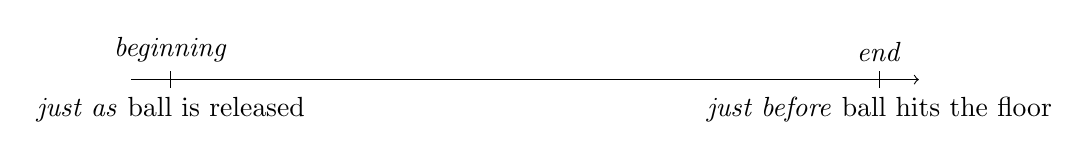
\begin{tikzpicture}
    % draw horizontal line   
    \draw[->] (0,0) -- (10,0);

    % draw vertical lines
    \foreach \x in {0.5,9.5}
      \draw (\x cm,3pt) -- (\x cm,-3pt);

    % draw nodes
    \draw (0.5,0) node[below=3pt] {\emph{just as} ball is released} node[above=3pt] {\emph{beginning}};
    \draw (9.5,0) node[below=3pt] {\emph{just before} ball hits the floor} node[above=3pt] {\emph{end}};
\end{tikzpicture}
\end{center}

\begin{enumerate}
	\item Write on the board: What properties of the physical system (indicators) do you think change \textbf{significantly} between the initial and final state?  What energy systems are associated with those indicators?  Are these \emph{internal} or \emph{mechanical} energy systems, or both?
	\item Put a complete \EnergyDiagram{} on the board.  Show with an arrow if each energy system increases or decreases. Include initial and final values of the indicators.
	\item Write an algebraic representation of your \EnergyDiagram{} that expresses energy conservation in terms of the changes of energy of the relevant energy systems.  
\end{enumerate}

\WCD 

\subsection{Phenomenon: Dropping a coffee filter}

Drop a basket type coffee filter from a height of about two meters.  Release it oriented as shown in the figure.

\begin{center}
	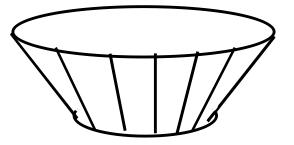
\includegraphics[width=0.25\textwidth]{act211-coffeefilter}

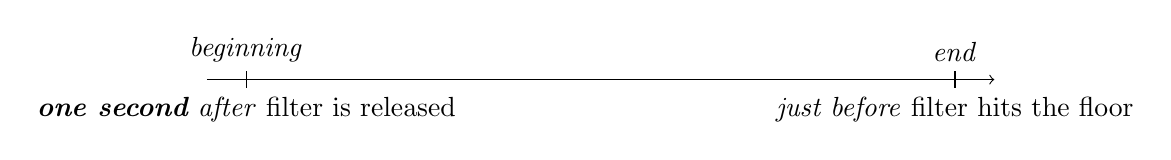
\begin{tikzpicture}
    % draw horizontal line   
    \draw[->] (0,0) -- (10,0);

    % draw vertical lines
    \foreach \x in {0.5,9.5}
      \draw (\x cm,3pt) -- (\x cm,-3pt);

    % draw nodes
    \draw (0.5,0) node[below=3pt] {\emph{\textbf{one second} after} filter is released} node[above=3pt] {\emph{beginning}};
    \draw (9.5,0) node[below=3pt] {\emph{just before} filter hits the floor} node[above=3pt] {\emph{end}};
\end{tikzpicture}
\end{center}

\begin{enumerate}
	\item Repeat part 1 above. Don't forget the last part of the question!
	\item Repeat parts 2 and 3 above.

\WCD 

\subsubsection*{Discuss in your group:}
	
	\item Which of the energy systems you have identified depend on only the \emph{magnitude} of the indicator and which depend on {\em both} the \emph{magnitude} and the \emph{sign} associated with that indicator? 
	\item How are your {\em particular models} for the golf ball and coffee filter different from each other?  Be specific.  What physical properties of the objects are responsible for this difference?
	
\end{enumerate}

\WCD 